\documentclass[12pt]{article}

\usepackage[a4paper, margin=1in]{geometry}
\usepackage{hyperref}
\usepackage{graphicx}
\usepackage{enumitem}
\usepackage{titlesec}
\usepackage{subcaption}
\usepackage{tikz}

\hypersetup{
    colorlinks=true,
    linkcolor=black,
    citecolor=black,
    urlcolor=blue   
}

\titleformat{\section}{\large\bfseries}{\thesection}{1em}{}
\titleformat{\subsection}{\normalsize\bfseries}{\thesubsection}{1em}{}

\title{SSL-PROJECT-REPORT \\ Snake Stack}
\author{Shiven Toshniwal \ Rishabh Iyer}
\date{May 2026}

\begin{document}

\maketitle

\tableofcontents
\newpage

\section{External libraries used with purpose}

\begin{itemize}[leftmargin=1.5em]
    \item Bootstrap 5 front end framework - For Styling \cite{Bootstrap}
    \item Math.random - For random generation of food items on the grid \cite{Math1}
    \item Math.floor - For random selection of coordinates as well as random selection of fruits \cite{Math2}
    \item Flask - Provides web server and routing capabilities \cite{Flask1} \cite{Flask2}
    \item datetime - Formats dates for the history.txt log
    \item os - Handles directory paths for serving static files
\end{itemize}

\section{Description of all features implemented}
    \begin{figure}[h]
    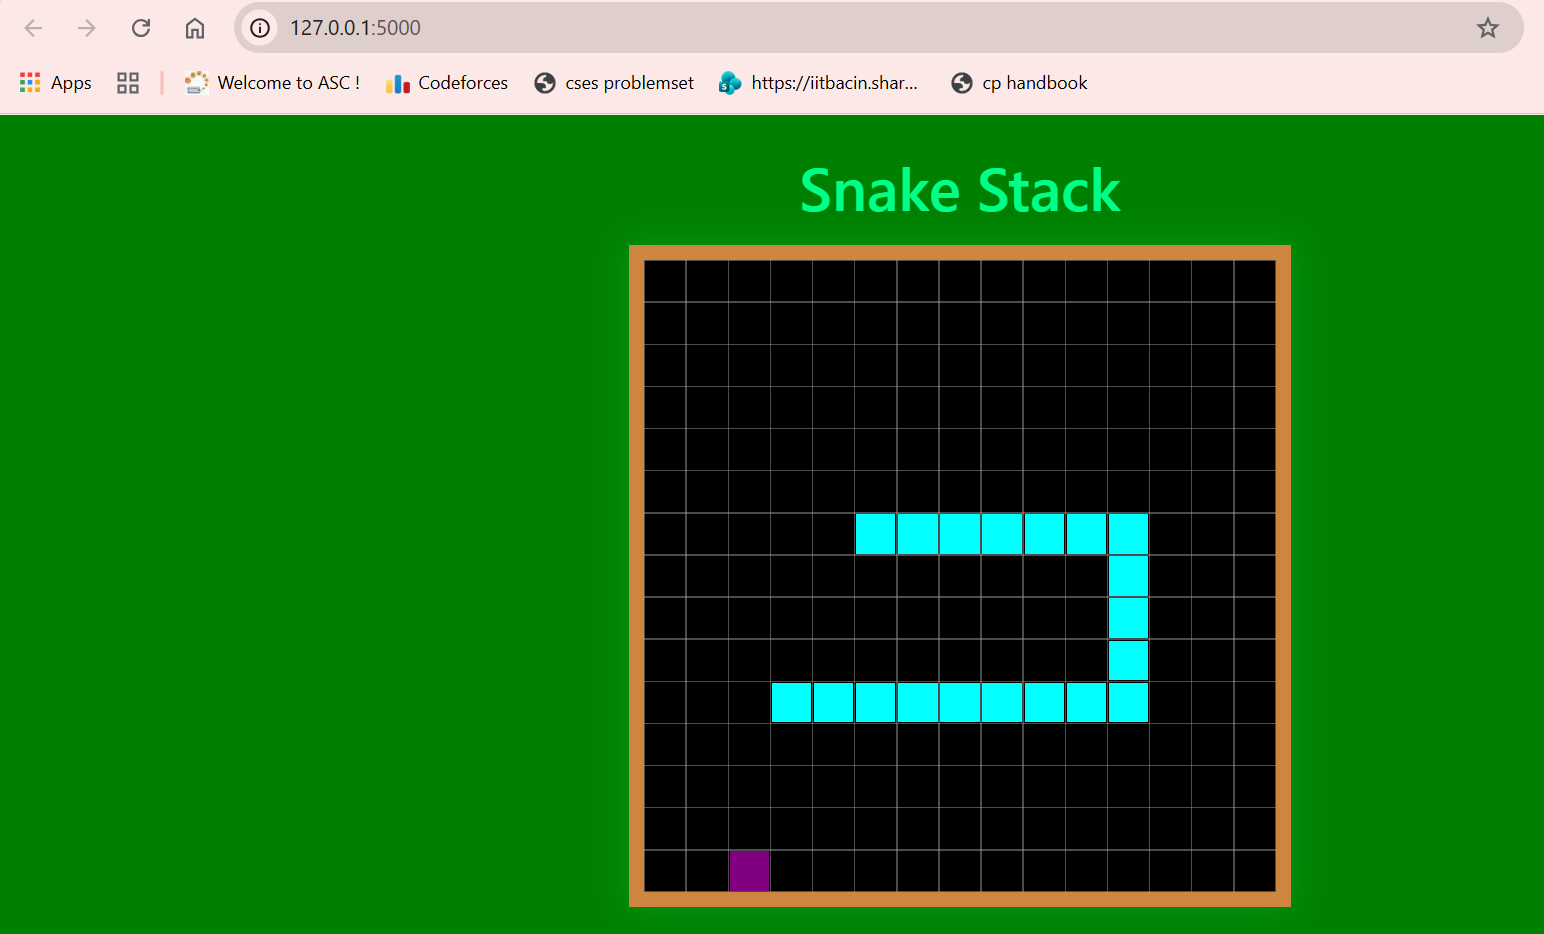
\includegraphics[width=\textwidth]{play.png}
    \caption{Ongoing game}
    \label{fig:play}
    \end{figure}
\subsection{Gameplay}

\begin{itemize}[leftmargin=1.5em]
    \item Welcome modal on starting game with start button and game information and asks for username which if not entered leads to display of alert message. (\ref{fig:start})
    \item Storing snake as an array of pairs of coordinates.
    \item Taking keyboard input to change position of head and popping last element of array.
    \item Storing food items as array of pairs of coordinates.
    \item Every 200ms, the boxes corresponding to coordinates of snake and foods are colored.(\ref{fig:play})
    \item Snake dies when the coordinates of head either coincide with another element of snake array or when it leaves the grid.
    \item 5 different types of fruits that the snake can feed on. One food item instantly appears when the previous is eaten.
    \item Incrasing length by retaining last "food.value" number of elements in snake array.
    \item Setting a 10s immunity timer in which the snake does not die on either hitting the wall or itself.
    \item Setting a 10s speed up by reducing the time interval between successive renderings of the board.
    \item Displays game-play statistics of current session.(\ref{fig:over})
\end{itemize}
\begin{figure}
    \begin{subfigure}[h]{0.4\textwidth}
    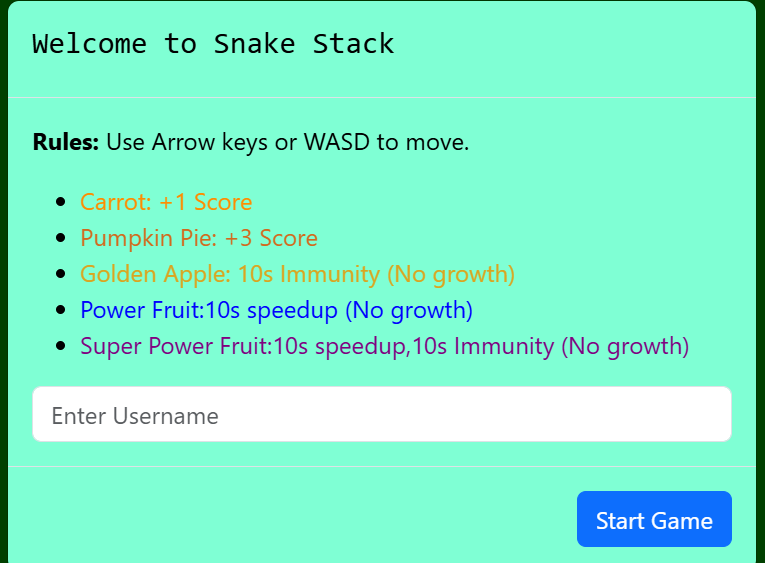
\includegraphics[width=\textwidth]{start.png}
    \caption{Game Start}
    \label{fig:start}
    \end{subfigure}
    \begin{subfigure}[h]{0.4\textwidth}
    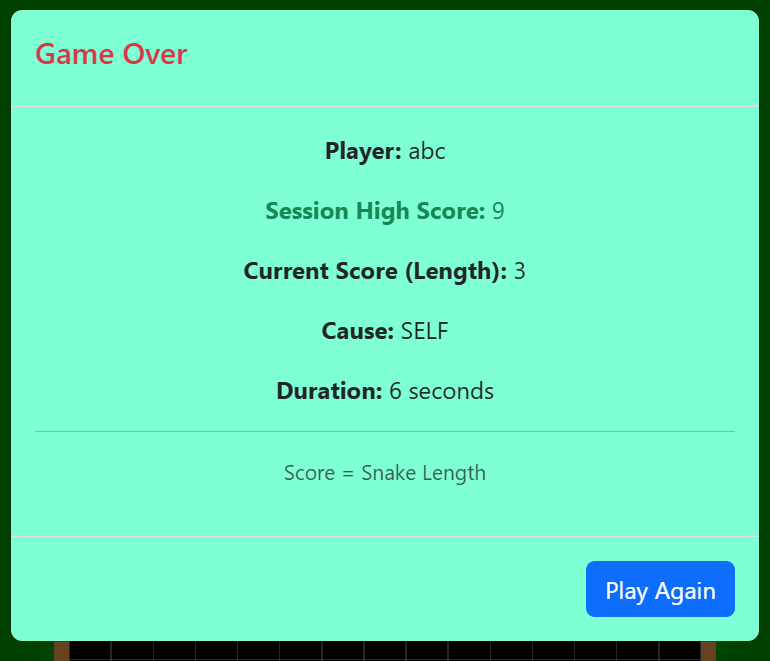
\includegraphics[width=\textwidth]{over.png}
    \caption{Game Over}
    \label{fig:over}
    \end{subfigure}
    \caption{User Interface}
\end{figure}
\subsection{Admin}

\begin{itemize}[leftmargin=1.5em]
    \item Checking for existence and emptiness of history.txt.
    \item Display menu driven interface
    \begin{itemize}
        \item Viewing Recent games
        \item Viewing analytics (Mean score/time)
        \item Deleting entries by username
        \item Log rotation in which history.txt is truncated to last 10 entries and backup is created in the form of .tar.gz file.
        \item Sorting by username or score (\ref{fig:admin1})
        \item Exit option
    \end{itemize}
    \item Handling invalid input and displaying error message.
    \item Using ANSI escape codes for colored output.
    (\ref{fig:admin2})
\end{itemize}
\begin{figure}
    \begin{subfigure}[h]{0.5\textwidth}
    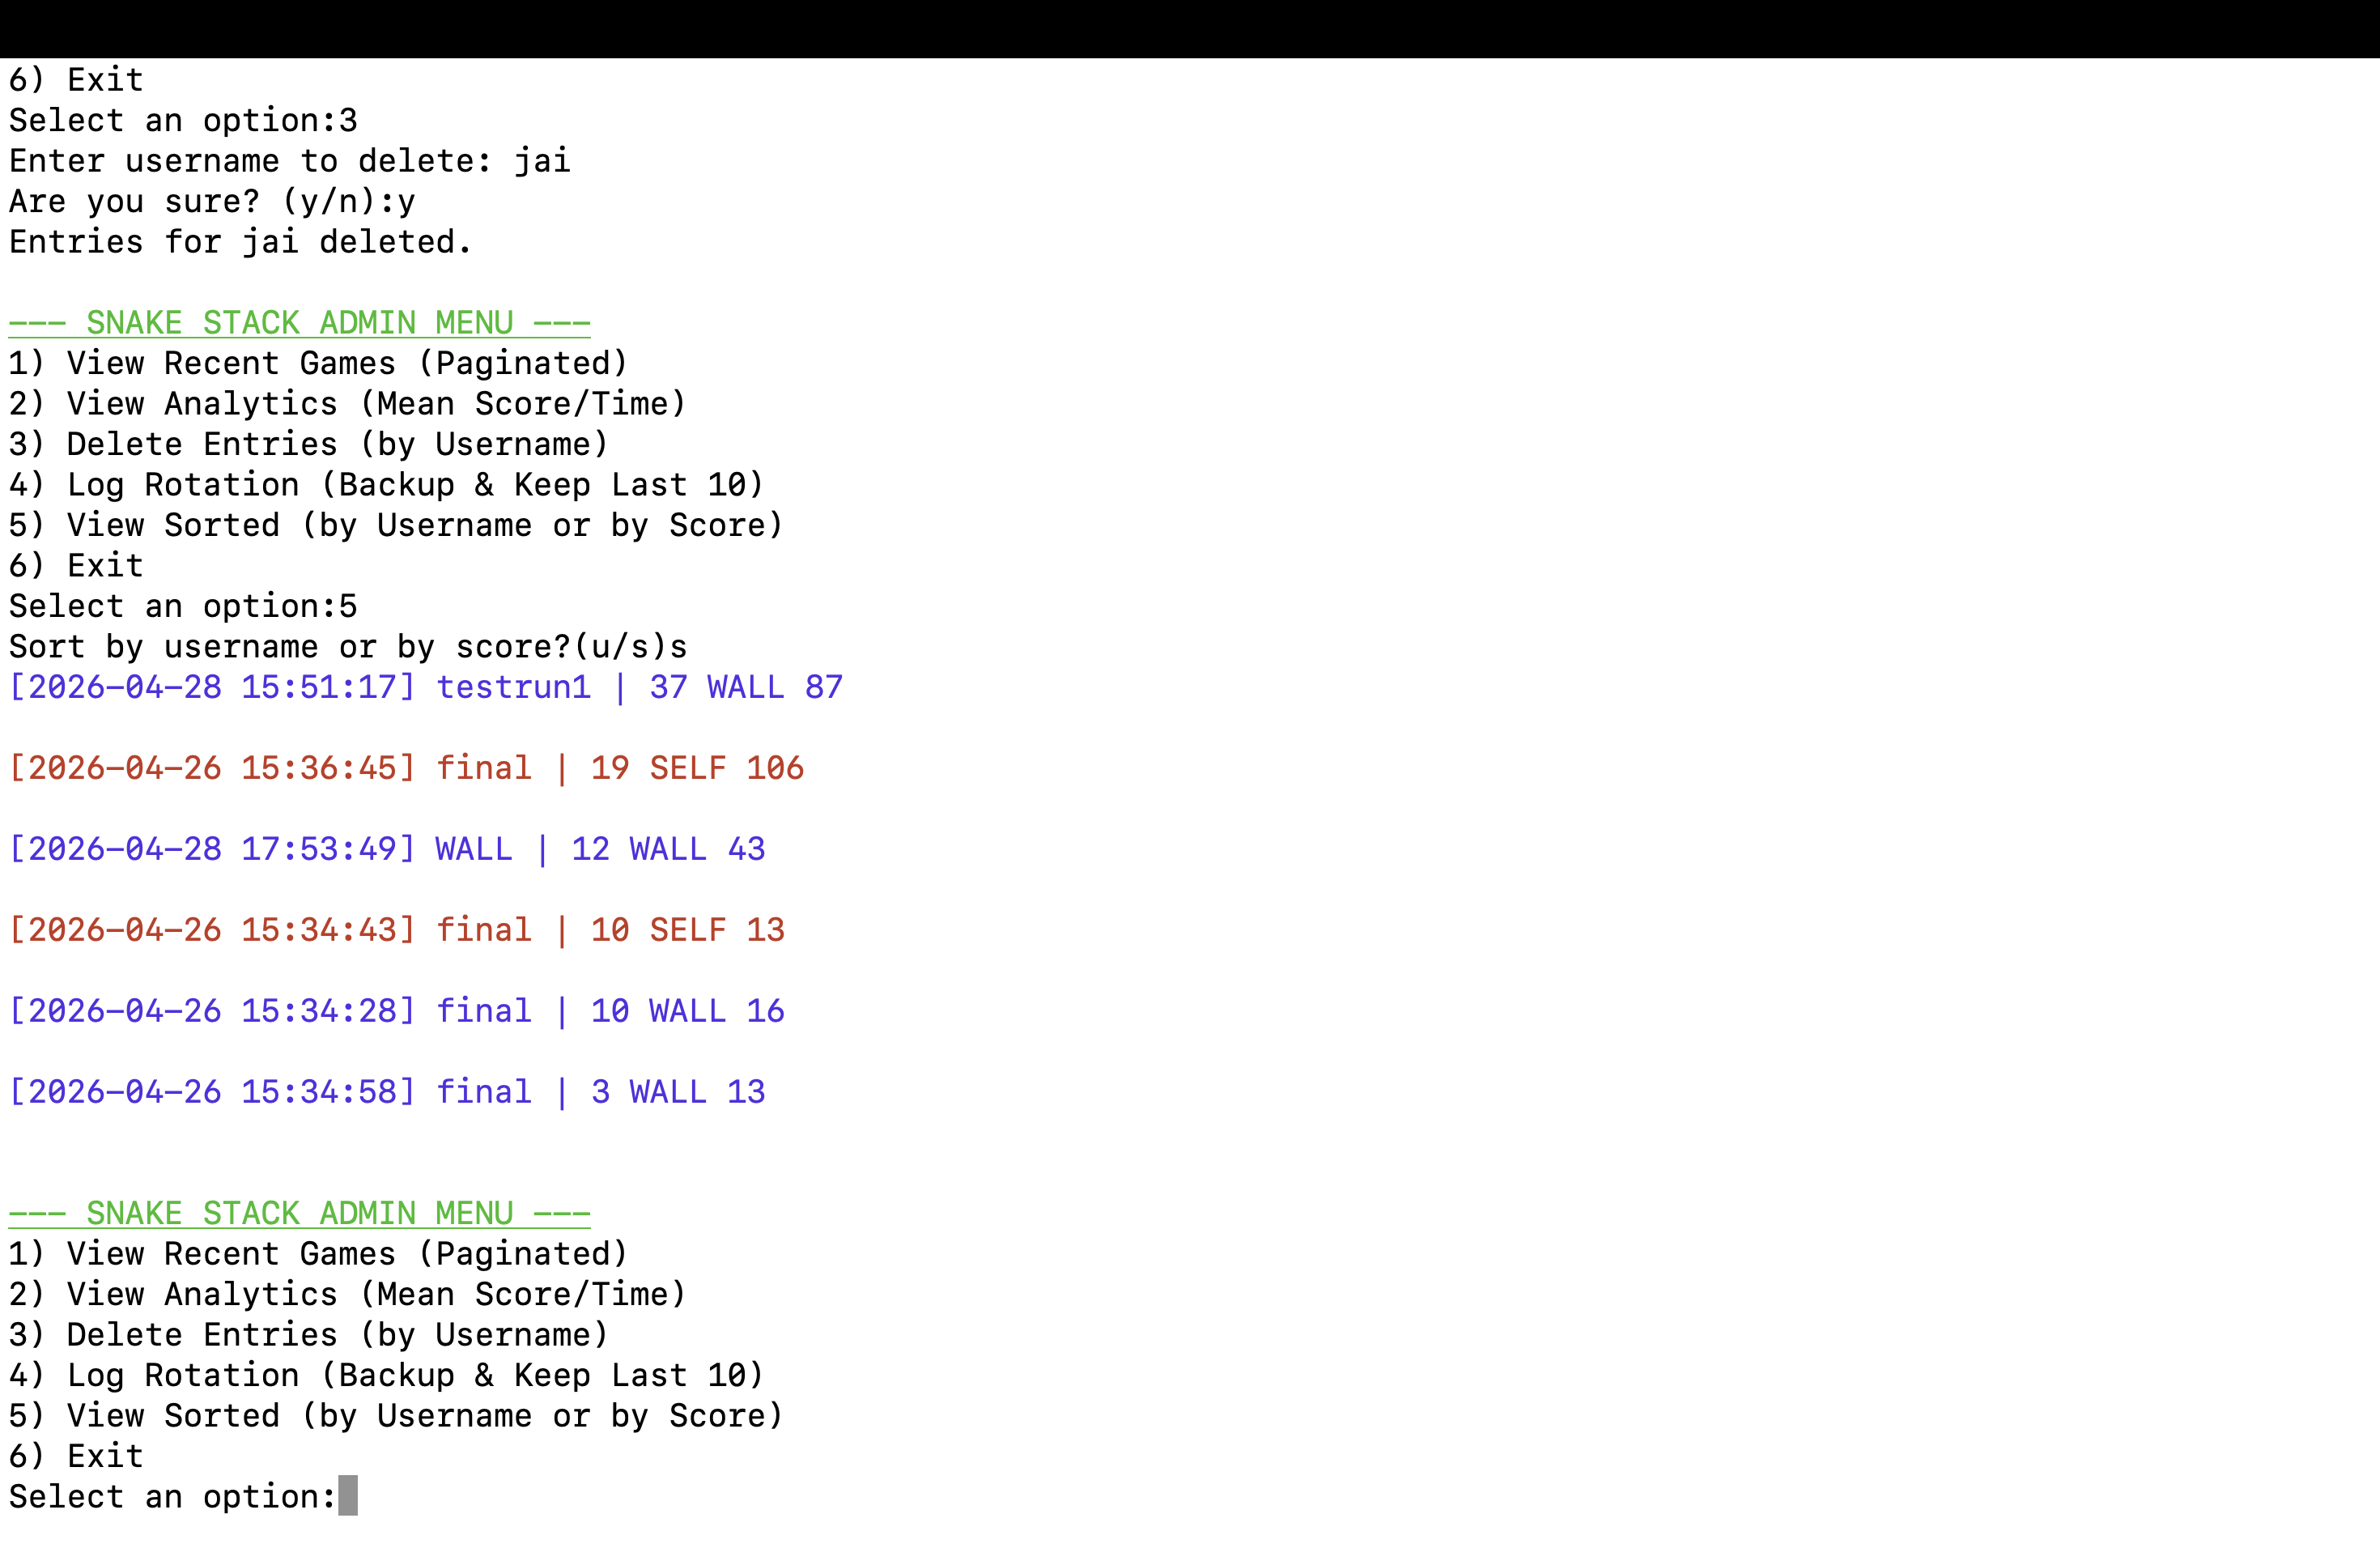
\includegraphics[width=\textwidth]{admin1.png}
    \caption{Sorting}
    \label{fig:admin1}
    \end{subfigure}
    \begin{subfigure}[h]{0.5\textwidth}
    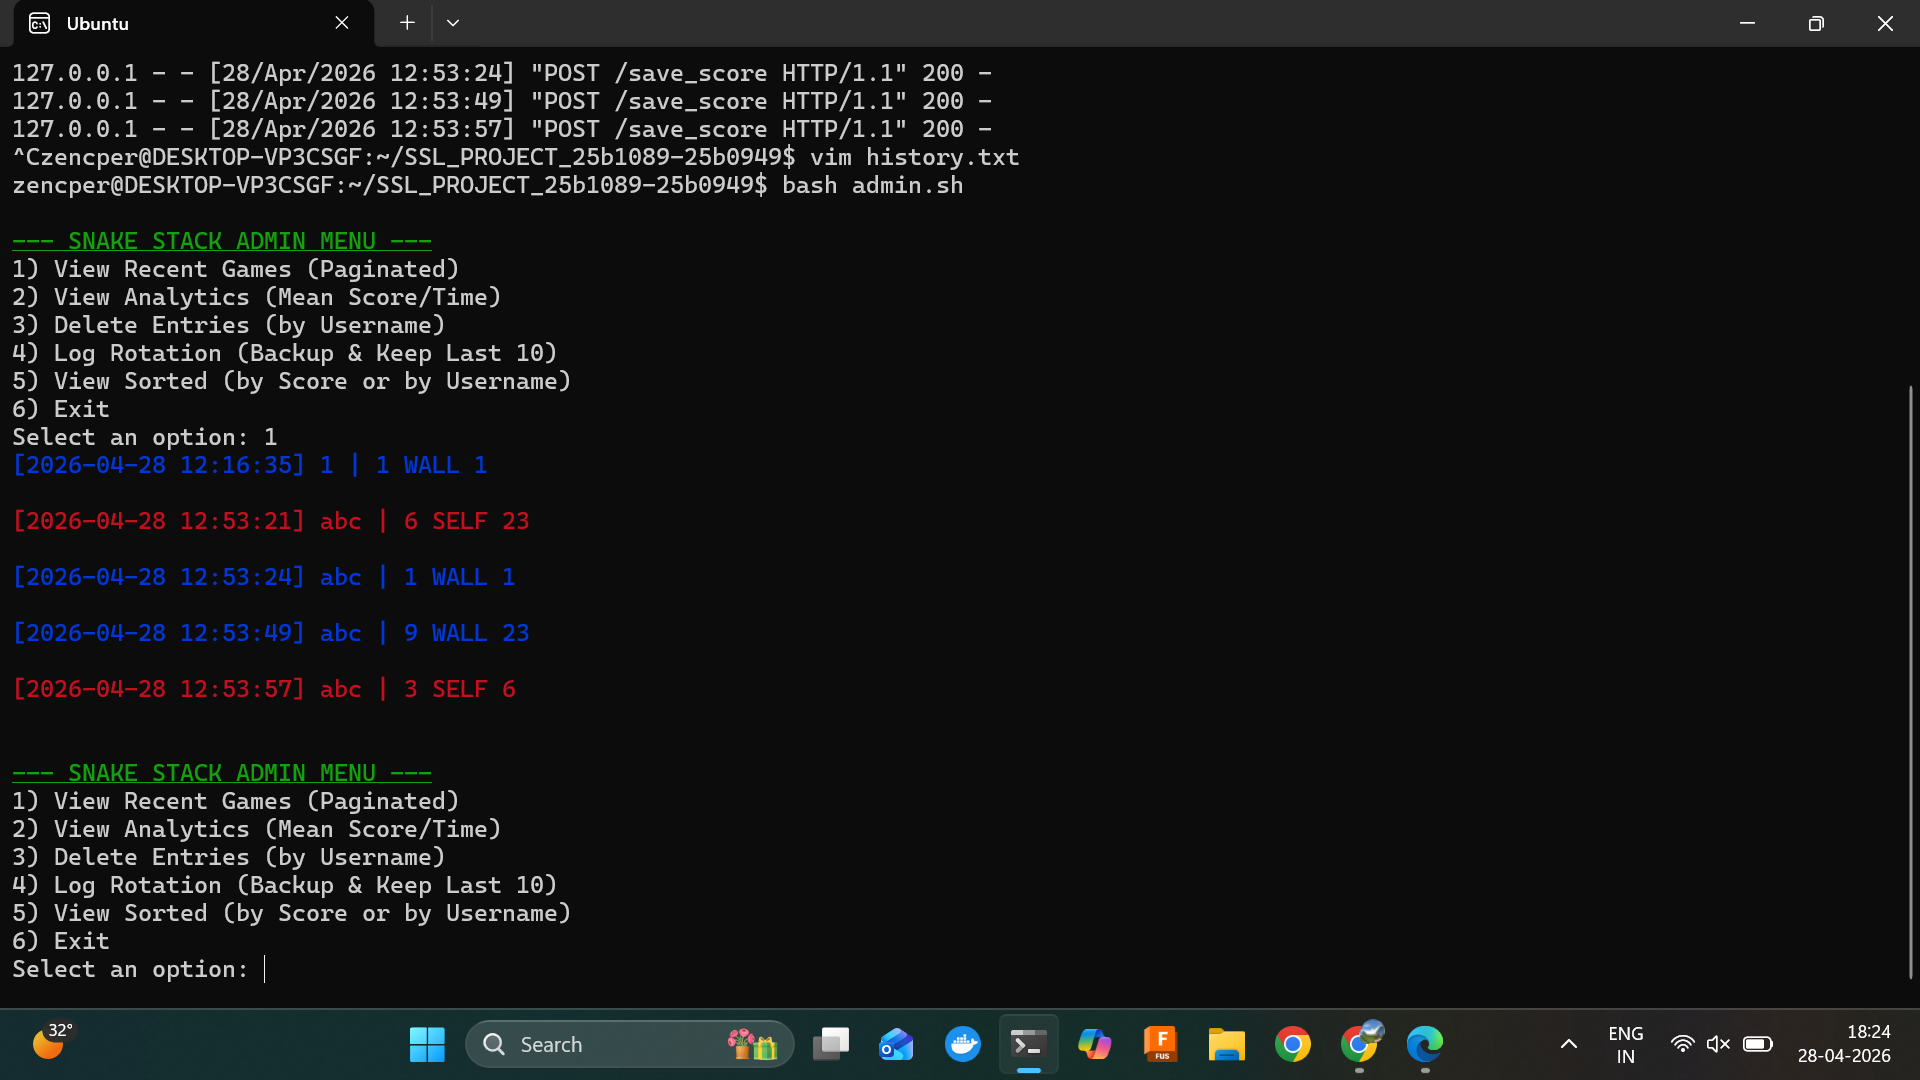
\includegraphics[width=\textwidth]{admin2.png}
    \caption{Recent games}
    \label{fig:admin2}
    \end{subfigure}
    \caption{Admin Features}
\end{figure}
\section{Directory structure \& how the 3 layers communicate }
\subsection{Directory structure}
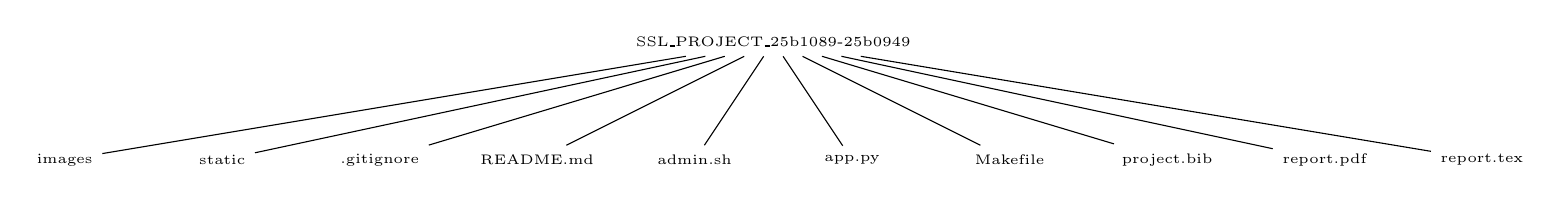
\begin{tikzpicture}[
    level 1/.style = {sibling distance=2 cm}, 
    every node/.style={font=\tiny}
]
\node {SSL\_PROJECT\_25b1089-25b0949}
    child { node {images} }
    child { node {static}}
    child {node {.gitignore}}
    child {node {README.md}}
    child {node {admin.sh}}
    child {node{app.py}}
    child {node{Makefile}}
    child {node {project.bib}}
    child {node {report.pdf}}
    child {node {report.tex}};
\end{tikzpicture}

\begin{tikzpicture}[
    level 1/.style = {sibling distance=3 cm}]  
\node {images} 
        child { node {admin1.png} }
        child { node {admin2.png} }
        child { node {over.png} }
        child {node {play.png} }
        child {node {start.png}};
\end {tikzpicture}

\begin{tikzpicture}[
    level 1/.style = {sibling distance=3 cm}]  
\node {static}
       child { node {api.js} }
        child { node {game.js} }
        child { node {index.html} }
        child {node {styles.css} }
        child {node {ui.js}};
\end {tikzpicture}

\subsection{How layers communicate}
At first, the user interacts with JavaScript front end framework. When the game ends, the front end sends the final score to Flask Server using fetch API. Request is POST with a JSON body. Inside app.py, the score is parsed, validated and appended to history.txt with timestamp. Managing history.txt and backup files by admin.sh. We have used bash commands like sed, awk, grep, cut, sort and case to create a menu driven interface with different options.

\subsection{Format for history.txt}

[timestamp] name \textbar~score  cause  duration \\ Chosen because with this format, sorting becomes easier and since game data is space separated, it can be handled by awk.

\section{Usage}
\begin{itemize}
\item Running game on server\\

Type 'python3 app.py' on command line.\\ Navigate to http://127.0.0.1:5000 on browser.\\ Enter username and press Start Game.\\ Can use arrow keys or WASD for snake motion.\\ Press Play Again to restart if game over
\item Running admin.sh \\

Type 'bash admin.sh' on command line.\\ Navigate menu by entering number corresponding to required option.\\ Where valid, enter required suboptions out of those visible
\end{itemize}
\section{Hurdles faced and how we overcame them}

\begin{itemize}[leftmargin=1.5em]
    \item Adjusting the display size of the grid and modal - By trial and error.
    \item Adjusting timers for changing speed of snake and setting immunity - Disabling existing loop and setting timer for running a new loop temporarily.
    \item Ensuring proper parsing and sorting of data in history.txt. For example, if username matches WALL or SELF - By using proper delimiters as per history.txt's format.
    \item Ensuring that a fruit does not generate on snake's body - Keeping in mind that the randomly generated fruit appears on the grid excluding all the coordinates inside snake array.
\end{itemize}

\section{What we would do in 10 extra hours}

\begin{itemize}[leftmargin=1.5em]
    \item Improve the graphics of both the snake and fruits.
    \item An option for the user to vary speed of snake, vary the types and numbers of fruits generated at a time.
\end{itemize}

\bibliographystyle{plain}
\bibliography{project}
\end{document}
